\documentclass{article}
\usepackage{main}
\usepackage[hyphens]{url}
\usepackage{graphicx}
\urlstyle{rm}
\def\UrlFont{\rm}
\usepackage{caption}
\usepackage[utf8]{inputenc}
\usepackage[T1]{fontenc}
\usepackage{booktabs}
\usepackage{amsfonts}
\usepackage{nicefrac}
\usepackage{microtype}
\usepackage{xcolor}
\usepackage{float}
\usepackage{amsmath}
\usepackage[normalem]{ulem}
\usepackage{cancel}
\usepackage{natbib}
\usepackage[none]{hyphenat}
\usepackage{array}
\usepackage{tabularx}
\usepackage{tikz}
\usepackage{pgfplots}
\pgfplotsset{compat=1.18}
\usepackage[hidelinks]{hyperref}
\allowdisplaybreaks
\newcolumntype{Y}{>{\raggedright\arraybackslash}X}
\newcommand{\HPWL}{\operatorname{HPWL}}
\newcommand{\E}{\mathbb{E}}


\title{Congestion-Aware Multi-Objective Macro Refinement\\Mid-Semester Research Proposal and Progress}
\renewcommand{\undertitle}{Mid-Semester Project Report}
\renewcommand{\shorttitle}{\small RL for Chip Placement: Mid-Semester Report}
\author{Aditya Birari\\2023A3PS0700P\\EEE Department
\And Pratyush Mohata\\2023A3PS0690P\\EEE Department}

\begin{document}
\maketitle

\begin{abstract}
This mid-semester report establishes our understanding of reinforcement learning (RL) for macro-placement refinement, reviews the relevant literature, and proposes a research direction. We select two complementary extensions: congestion-aware feedback and preference-conditioned multi-objective regulation. The proposed policy will refine an existing layout according to wirelength, regularity, and congestion preferences. Timing-aware feedback is a later possibility when suitable data and tools are available. Preliminary work includes source-code study, a small synthetic environment, initial congestion/Pareto utilities, and local execution of the released MaskRegulate policy. The proposed conditional regulator has not yet been trained or evaluated. The present deliverable is a problem formulation and an initial implementation foundation for the remaining project.
\end{abstract}

\section{Problem understanding and motivation}

\subsection{What is chip placement?}
A circuit netlist specifies components and their electrical connections. Placement assigns these components physical coordinates on a chip canvas before routing connects their pins. Macros are large blocks, such as memories; standard cells are smaller logic instances. Macro locations strongly influence the space left for standard cells and interconnect. A placement with short estimated connections can still obstruct routing or create local demand hotspots. Our project refines the locations of existing blocks while keeping their functionality and dimensions fixed.

Represent the circuit as a hypergraph $G=(V,E)$, where vertices represent components and each hyperedge connects the pins of one net. A macro $i$ has lower-left coordinates $(x_i,y_i)$, dimensions $(w_i,h_i)$, and pin offsets. Its pins translate with the macro. On a canvas of width $W$ and height $H_d$, coordinates must satisfy
\begin{equation}
0\leq x_i\leq W-w_i,\qquad 0\leq y_i\leq H_d-h_i.
\end{equation}
Rectangles must not overlap, and fixed objects and blockages must be respected. Real physical flows also impose rules such as halos, orientations, and site alignment. Choices are coupled: moving one macro changes several nets and the space available to other objects. The feasible placement problem is therefore a large combinatorial search.

\subsection{Objectives and the limitations of proxies}
The common wirelength proxy is weighted half-perimeter wirelength (HPWL):
\begin{equation}\label{eq:hpwl}
H(P)=\sum_{e\in E}\omega_e\left[
\max_{p\in e}p_x-\min_{p\in e}p_x+
\max_{p\in e}p_y-\min_{p\in e}p_y\right].
\end{equation}
Here $P$ denotes a placement, $\omega_e\geq0$ is the weight of net $e$, and $(p_x,p_y)$ are pin coordinates. For pins $(1,1),(4,2),(3,5)$, an unweighted net contributes $3+4=7$. HPWL measures bounding-box extent, not an actual routed path. With affine pin translations it is convex but nonsmooth in unrestricted coordinates; non-overlap and other placement constraints make the overall problem nonconvex.

\emph{Congestion} arises when local routing demand competes for limited resources. A fast demand estimate, global-route overflow, and detailed-routing violations are different measurements. \emph{Regularity} is the reference method's preference for organized peripheral macro geometry; it is useful guidance rather than proof of low congestion. \emph{PPA} means power, performance, and area. Lower HPWL or a demand proxy alone does not demonstrate improved timing, power, or area. Those claims require a suitable physical evaluation flow \citep{openroad}.

\subsection{Why use an RL regulator?}
A constructive RL placer assigns coordinates before all future positions are known. A regulator begins with a complete placement and adjusts it, so a move can be assessed against known positions of connected objects. This provides more informative feedback and allows revision of an existing solution. Analytical tools such as DREAMPlace can provide starting placements \citep{dreamplacecode}.

Refinement remains challenging: a useful move may worsen one objective while improving another, a learned policy may depend on its initializer, and a cheap proxy can disagree with downstream routing. These issues motivate our selected direction: teach a regulator to respond to explicitly stated objective preferences and test whether its improvements remain meaningful.

\section{Literature review and research gap}

\subsection{From constructing placements to refining them}
\citet{lai2022maskplace} use visual masks, action constraints, and dense wirelength feedback for constructive macro placement. Thus, masks and frequent rewards are established ideas. \citet{lai2023chipformer} study transferable placement through offline decision transformers; this motivates separating frozen-policy transfer from target-circuit adaptation. Non-RL refinement is also relevant: IncreMacro demonstrates that incremental adjustment and peripheral guidance can improve a layout without an RL policy \citep{pu2024incremacro}.

\citet{xue2024maskregulate} change RL's role from macro placer to macro regulator. MaskRegulate refines an existing placement using Proximal Policy Optimization (PPO), an RL training algorithm, together with wirelength information and regularity feedback. Its original study already includes unseen-circuit evaluation, training on \texttt{superblue1/3/4/5} and testing on \texttt{superblue7/10/16/18}. Therefore, testing on an unseen circuit alone would not be a sufficient new contribution.

The released implementation also has important details for reproduction. OLD/NEW occupancy maps allow moves into locations of macros that have not yet been adjusted; intermediate overlap can occur, so complete-pass outputs need independent checks. Quantities are already normalized. Our extension must preserve and document these conventions rather than compare against an invented unnormalized or always-legal baseline \citep{maskregulatecode}.

\subsection{Diffusion placement as a comparison point}
\citet{lee2025diffusion} train a graph-conditioned diffusion model on synthetic circuit--layout pairs and generate placements through coordinate denoising. Guidance and legalization contribute to inference-time quality. This provides a different route to transferable placement, but it is a generator rather than an existing-layout refiner. Its published results and MaskRegulate's results use different settings and cannot be treated as a controlled direct comparison. Diffusion is useful context for the project; integrating another full framework is outside the present mid-semester scope.

\subsection{Congestion and multi-objective prior art}
Rectangular Uniform wire DensitY (RUDY) is an established fast routing-demand estimator \citep{spindler2007rudy}. It distributes estimated net demand across pin bounding rectangles. Dividing the canvas into grid cells, called bins, produces a spatial map of estimated demand. A lightweight implementation without routing layers, capacities, and obstruction handling is a RUDY-style \emph{demand proxy}, not a routed-congestion measurement.

\citet{chang2022moppo} already propose preference-conditioned multi-objective RL chip placement using a multi-objective PPO method (MOPPO). Consequently, training one model with inference-time weights is not new by itself. Newer placement studies also incorporate expert guidance or alternative generative formulations \citep{gao2026expertise,xie2026flowplace}. Our contribution must be a well-motivated refinement extension with appropriate evaluation, rather than a first-ever claim about multi-objective placement.

\begin{table}[h]
\caption{Main literature lessons informing the proposed project.}
\label{tab:literature}
\small
\begin{tabularx}{\linewidth}{@{}p{0.24\linewidth}YY@{}}
\toprule
Work & Relevant idea & Implication\\
\midrule
MaskPlace / ChiPFormer & Mask-based RL / transfer & Established foundations; define the transfer setting.\\
MaskRegulate & Refine an existing layout & Principal baseline; generalization already studied.\\
ChipDiffusion & Synthetic-trained generation & Contextual comparison; different pipeline and inputs.\\
RUDY / MOPPO & Demand estimation / preferences & Both ingredients have prior art.\\
IncreMacro & Classical refinement & Strong non-learning controls are necessary.\\
\bottomrule
\end{tabularx}
\end{table}

\subsection{Research gap and the two proposed extensions}
This project proposes to extend MaskRegulate in two connected ways.

\paragraph{Congestion-aware reward.}
Add a fast estimate of routing-demand hotspots to the regulator's existing wirelength and regularity objectives. The policy would receive positive feedback when a refinement reduces the combined cost, so training considers estimated congestion explicitly. Timing-aware feedback is a possible later extension, contingent on genuine timing data and a working analysis flow.

\paragraph{Preference-conditioned multi-objective refinement.}
Give the regulator an input vector specifying the desired balance between wirelength, regularity, and congestion. Instead of using only one fixed balance, the same trained policy would be queried with different preferences to generate alternative layouts. Feasible alternatives would then be filtered into an empirical nondominated set: no other sampled feasible layout is no worse on all objectives and better on at least one.

\textbf{Research question.} Can one congestion-aware, preference-conditioned regulator produce useful wirelength--regularity--congestion trade-offs on unseen circuits, and do improvements in its demand proxy agree with routing-based measurements? The proposed contribution is the evaluated combination of these extensions in placement refinement. The preliminary work reported here does not yet answer this question.

\section{Proposed research direction and problem formulation}

\subsection{Input, output, and objectives}
The proposed method takes a circuit, geometry/constraints, an initial placement $P_0$, a compute budget, and a preference vector. It returns a checked feasible refinement. The core minimized objective vector will be
\begin{equation}
\mathbf f(P)=\big(H(P),R(P),C(P)\big),\qquad
\boldsymbol\lambda=(\lambda_H,\lambda_R,\lambda_C)\geq0,\quad \sum_j\lambda_j=1.
\end{equation}
$H$ is pin HPWL; $R$ retains MaskRegulate's regularity definition; $C$ summarizes high-demand bins of a declared RUDY-style map. We propose the mean of the top ten percent of bins, rather than whole-grid mean demand, because whole-grid demand largely follows total estimated wirelength. Bin resolution, degenerate-net handling, net demand, and normalization will be fixed and verified.

The main implementation will begin with congestion-aware feedback. Timing is an optional later extension: criticality-weighted HPWL or periodic timing analysis requires genuine criticalities, libraries, constraints, and an analysis flow. It will not be presented as measured timing improvement merely because a geometric proxy decreases.

\subsection{Preference-conditioned policy and reward}
The reference environment supplies placement, wirelength, and regularity masks for macro adjustment. The actor selects a macro's destination, while the critic estimates the expected future return used during training. We propose adding congestion information and the preference vector to both networks. Changing only the reward would not let identical observations select different actions for different preferences. PPO is the planned learning algorithm, following MaskRegulate \citep{schulman2017ppo}.

For fixed episode scales $s_j=\max(f_j(P_0),\varepsilon_j)>0$, define
\begin{equation}\label{eq:reward}
J_{\boldsymbol\lambda}(P)=\sum_j\lambda_j\frac{f_j(P)}{s_j},
\qquad r_t=J_{\boldsymbol\lambda}(P_t)-J_{\boldsymbol\lambda}(P_{t+1}).
\end{equation}
Here $J_{\boldsymbol\lambda}$ is the preference-weighted cost, $r_t$ is the reward for moving from $P_t$ to $P_{t+1}$, and each $\varepsilon_j$ is a positive minimum scale preventing division by zero. These minimum scales will be fixed using training/validation, and all methods will share the same references on a given start. An episode is one finite sequence of refinement moves; its preferences remain fixed. With undiscounted fixed-horizon return, the reward sum equals initial-minus-final scalar cost. MaskRegulate's discounting or other shaping changes this relationship and will be documented.

For example, $(0.7,0.2,0.1)$ emphasizes wirelength, whereas $(0.2,0.1,0.7)$ emphasizes the congestion proxy. The intended benefit is to query the same trained regulator for different trade-offs. Feasibility is a constraint: a preference cannot justify an illegal returned placement. Native passwise masks will be preserved and final endpoints checked independently.

\begin{figure}[h]
\centering
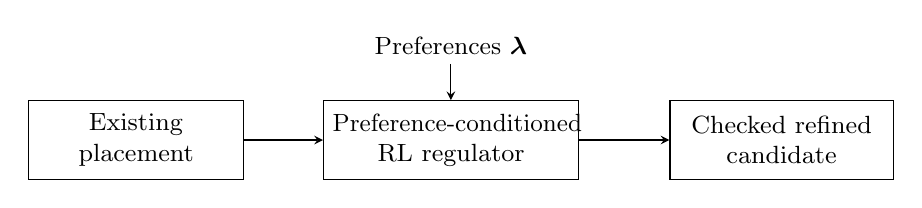
\begin{tikzpicture}[font=\small,>=stealth]
\node[draw,align=center,text width=2.5cm,minimum height=1cm] (a) at (0,0) {Existing\\placement};
\node[draw,align=center,text width=3cm,minimum height=1cm] (b) at (4,0) {Preference-conditioned\\RL regulator};
\node[draw,align=center,text width=2.6cm,minimum height=1cm] (c) at (8.2,0) {Checked refined\\candidate};
\node[align=center] (w) at (4,1.2) {Preferences $\boldsymbol\lambda$};
\draw[->] (a) -- (b); \draw[->] (b) -- (c); \draw[->] (w) -- (b);
\end{tikzpicture}
\caption{Proposed core pipeline. Repeating inference for a declared preference set will provide candidate trade-offs. Training and systematic evaluation of this conditional regulator are future work.}
\end{figure}

\subsection{What ``Pareto'' will mean here}
A feasible placement dominates another if it is no worse on every objective and strictly better on at least one. We will remove dominated and duplicate outputs to obtain an \emph{empirical nondominated set}. A finite weighted-sum sweep does not guarantee recovery of the entire Pareto frontier, particularly unsupported nonconvex regions \citep{das1997weightedsum}.

The planned hypotheses are: congestion feedback improves the available trade-offs; preference conditioning is useful relative to fixed-weight models and search; and proxy rankings remain sufficiently consistent with routing-based evaluation. Each hypothesis needs experiments after the mid-semester stage.

\section{Preliminary work completed}

\subsection{Understanding and initial implementation}
We have reviewed the anchor papers and relevant prior art, inspected the released MaskRegulate code, and formulated the selected extension. A small NumPy environment implements rectangles, pin HPWL, feasibility checks, and dense improvement rewards. An educational linear REINFORCE policy checks the learning/evaluation scaffold \citep{williams1992reinforce}; it is distinct from the original PPO model.

For the new direction, initial utilities compute a RUDY-style map, top-decile demand, normalized objective costs, and nondominated filtering. A six-preference greedy smoke sweep produced 48 toy runs across four synthetic netlists and two starts. Checks cover finite demand, demand integration, degenerate nets, feasibility, dominance, and reward telescoping. These are functionality checks and a control implementation; a learned preference-conditioned regulator is not implemented yet.

\subsection{Initial execution of the MaskRegulate reference}
On this PC, we installed an isolated CPU environment and strictly loaded the released checkpoint into the original actor/critic. Diagnostic inference verified valid action probabilities and masking. An adapted component harness also completed one 512-move policy pass and one greedy pass on the selected-module representation of \texttt{superblue18}, with independently checked rectangle feasibility.

This is preliminary baseline execution. DREAMPlace initialization/evaluation was bypassed explicitly, a legal reference-derived start was supplied, and no training occurred. The full original entry point remains unavailable without the compiled backend. The component trial also exposed a discrepancy in the auxiliary macro-HPWL reporter; a per-net audit identified omitted nets on this nonsquare case. This motivates independent metric checks and is not a conclusion about the paper's separate global-HPWL results.

\begin{table}[h]
\caption{Mid-semester status: completed foundations versus proposed work.}
\small
\begin{tabularx}{\linewidth}{@{}p{0.26\linewidth}YY@{}}
\toprule
Component & Current status & Next step\\
\midrule
Literature/formulation & Congestion-aware, preference-conditioned refinement proposed & Refine implementation details with feedback.\\
Toy objective/environment & Initial code and smoke checks & Connect checked congestion feedback to native RL.\\
Original policy & Checkpoint and component execution & Establish a full backend-compatible baseline.\\
Conditional PPO regulator & Proposed & Add preference inputs and train a small pilot.\\
Generalization/routing & Not evaluated & Run controlled held-out and downstream studies.\\
\bottomrule
\end{tabularx}
\end{table}

Detailed logs, raw toy results, adapter limitations, and rerun commands are retained in the repository rather than treated as final project results. No completed conditional-model training, real-circuit generalization study, routing/timing validation, or PPA improvement is claimed.

\section{Planned evaluation and work after mid-semester}
The next steps are to establish the native baseline, validate the congestion evaluator, train a fixed-weight congestion-aware regulator, and then add preference conditioning. This order separates reward changes from conditioning changes. GPU access is available on another machine; the local PC currently runs CPU component checks.

Training, validation, and test designs will be separated by circuit family. Checkpoints and hyperparameters will use validation only. Planned controls include the original regulator, a fixed-weight congestion-aware model, fixed-weight specialists, no refinement, and greedy/simulated-annealing refinement. We will compare candidate sets under the same \emph{total} deployment budget, including proxy and backend costs, rather than giving a preference sweep uncounted extra runs.

Planned measurements include HPWL, regularity, the demand proxy, endpoint feasibility, runtime, and empirical-set quality. Hypervolume, a measure of the objective-space region dominated by the sampled layouts relative to a reference point, will use common scales and a reference fixed without final-test outcomes. Component-wise comparisons (ablations) will isolate congestion reward, congestion observation, and preference conditioning. Where compatible data/tools permit, a small preselected subset will be checked for global-route congestion and timing at a common stage \citep{openroadgpl,openroadgrt}. Such evaluation is planned, not completed.

\begin{table}[h]
\caption{Indicative plan for the remaining two months.}
\small
\begin{tabularx}{\linewidth}{@{}p{0.17\linewidth}Y@{}}
\toprule
Period & Planned milestone\\
\midrule
Weeks 1--2 & Backend-compatible baseline and independently verified congestion metric.\\
Weeks 3--4 & Fixed-weight congestion model and a small preference-conditioned PPO pilot.\\
Weeks 5--6 & Held-out circuits, search/specialist controls, and focused ablations.\\
Weeks 7--8 & Downstream audit where feasible, failure analysis, and final report.\\
\bottomrule
\end{tabularx}
\end{table}

The mid-semester contribution is therefore a clear understanding of the problem, a literature-grounded research direction, a proposed formulation, and initial implementation evidence. Whether the proposed model provides better trade-offs remains the question for the rest of the project.

\paragraph{Project repository.}
\url{https://github.com/BirariAditya/chip-refinement-generalization}.
The private repository contains literature notes, source, preliminary records, and the proposed experimental protocol.

\begingroup
\small
\setlength{\bibsep}{3pt}
\bibliography{references}
\bibliographystyle{apalike}
\endgroup
\end{document}
